\subsection{Permutations and combinations}

\begin{theorem*}
  The number of $k$-tuples that can be formed from $\{1, 2, \ldots, n\}$ is
  \begin{align*}
    P(n, k) = n_{(k)} = n(n-1)(n-2)\cdots(n-k+1).
  \end{align*}
  The number of sets of size $k$ that can be formed from $\{1, 2, \ldots, n\}$ is
  \begin{align*}
    C(n, k) = {n \choose k} = \frac{P(n, k)}{k!}.
  \end{align*}
\end{theorem*}

\subsection{Binomial theorem}
\begin{align*}
  (a + b)^n = \sum_{k=0}^n{n \choose k}a^{n-k}b^k
\end{align*}

\subsection{Triangle inequalities}

\begin{theorem*}
  Let $a, b \in \R$ with $a \neq b$ and $a, b \neq 0$. Using $+$, $-$ and $|\cdot|$ we can generate the
  following 4 real numbers:
  \begin{align*}
    -\big(|a| + |b|\big) ~~~ < ~~~
    -\big||a| - |b|\big| ~~~ < ~~~
    0                    ~~~ < ~~~
    \big||a| - |b|\big|  ~~~ < ~~~
    |a| + |b|.
  \end{align*}
  \begin{itemize}
  \item $a + b$ and $a - b$ can equal any of them.
  \item $|a + b|$ and $|a - b|$ can equal either of the two positive numbers.
  \item $|a| - |b|$ can equal either of the two ``inner'' numbers.
  \end{itemize}
  ~\\~\\
  If we allow $a = b$ with $ a \neq 0, b \neq 0$ then
  \begin{align*}
    -\big(|a| + |b|\big) ~~~ < ~~~
    -\big||a| - |b|\big| ~~~ \red{\leq} ~~~
    0                    ~~~ \red{\leq} ~~~
    \big||a| - |b|\big|  ~~~ < ~~~
    |a| + |b|.
  \end{align*}
  If we allow $a = 0$ and $b = 0$ with $a \neq b$ then
  \begin{align*}
    -\big(|a| + |b|\big) ~~~ \red{\leq} ~~~
    -\big||a| - |b|\big| ~~~ < ~~~
    0                    ~~~ < ~~~
    \big||a| - |b|\big|  ~~~ \red{\leq} ~~~
    |a| + |b|;
  \end{align*}
  If we allow $a = b$ including $a = b = 0$ then
  \begin{align*}
    -\big(|a| + |b|\big) ~~~ \red{\leq} ~~~
    -\big||a| - |b|\big| ~~~ \red{\leq} ~~~
    0                    ~~~ \red{\leq} ~~~
    \big||a| - |b|\big|  ~~~ \red{\leq} ~~~
    |a| + |b|;
  \end{align*}
\end{theorem*}

\subsection{The quadratic formula}

\begin{theorem*}
  The roots of $ax^2 + bx + c = 0$ are $x = \frac{-b \pm \sqrt{b^2 - 4ac}}{2a}$.
\end{theorem*}

\begin{proof}
  \begin{align*}
    x^2 + \frac{b}{a}x + \frac{c}{a}                        &= 0\\
    \(x + \frac{b}{2a}\)^2 - \frac{b^2}{4a^2} + \frac{c}{a} &= 0 ~~~~~~~~~~~~~~~~~~~~~\text{``completing the square"}\\
    x &= -\frac{b}{2a} \pm \sqrt{\frac{b^2}{4a^2} - \frac{4ac}{4a^2}}\\
                                                            &= \frac{-b \pm \sqrt{b^2 - 4ac}}{2a}.
  \end{align*}
\end{proof}

\subsection{Geometric series}
\begin{theorem*}
  $a_n := \sum_{k=0}^nr^n = \frac{~~~~1 - r^{n+1}}{1 - r}$.

  Therefore if $r < 1$ then $\lim_{n \to \infty} a_n = \frac{1}{1 - r}$.
\end{theorem*}
\begin{proof}
  \begin{align*}
    a_n          &= \sum_{k=0}^nr^n = 1 + r + r^2 + \ldots + r^n\\
    a_n - ra_n  &= 1 - r^{n+1}\\
    a_n          &= \frac{~~~~1 - r^{n+1}}{1 - r}
  \end{align*}
\end{proof}
\begin{remark*}
  Note that $a_{n+1} = 1 + ra_n$.
\end{remark*}

\subsection{Partial fractions}

\red{TODO}

\subsection{Even and odd functions}

\begin{definition*}
  A function (over an additive group?) is even if and only if $f(-x) = f(x)$ for all $x$.

  A function (over an additive group?) is odd if and only if $f(-x) = -f(x)$ for all $x$.
\end{definition*}

Functions can be neither even nor odd.

\begin{claim*}
  A polynomial $p(x)$ is even if an only if it has only even powers of $x$.

  A polynomial $p(x)$ is odd if an only if it has only odd powers of $x$.
\end{claim*}

\subsection{$\sqrt{2}$ is irrational}
\begin{theorem*}
  $\sqrt{2}$ is irrational.
\end{theorem*}

\begin{proof}
  Suppose $\sqrt{2} \in \Q$. Then $\sqrt{2}$ can be written as $\frac{a}{b}$ where $a, b \in \Z$
  have no common factor (aka coprime, aka mutually prime).

  Then $2 = \frac{a^2}{b^2}$, so $a^2$ is even.

  Therefore $a$ is even.

  Let $a = 2c$. Then $b^2 = \frac{4c^2}{2} = 2c^2$, so $b^2$ is even.

  Therefeore both $a$ and $b$ are even, which is a contradiction.

  Therefore $\sqrt{2} \notin \Q$.
\end{proof}

\begin{remark*}
  It remains to be proved that $\sqrt{2}$ exists in $\R$. See \ref{existence-of-root-2}.
\end{remark*}

\subsection{Misc}
\begin{mdframed}
  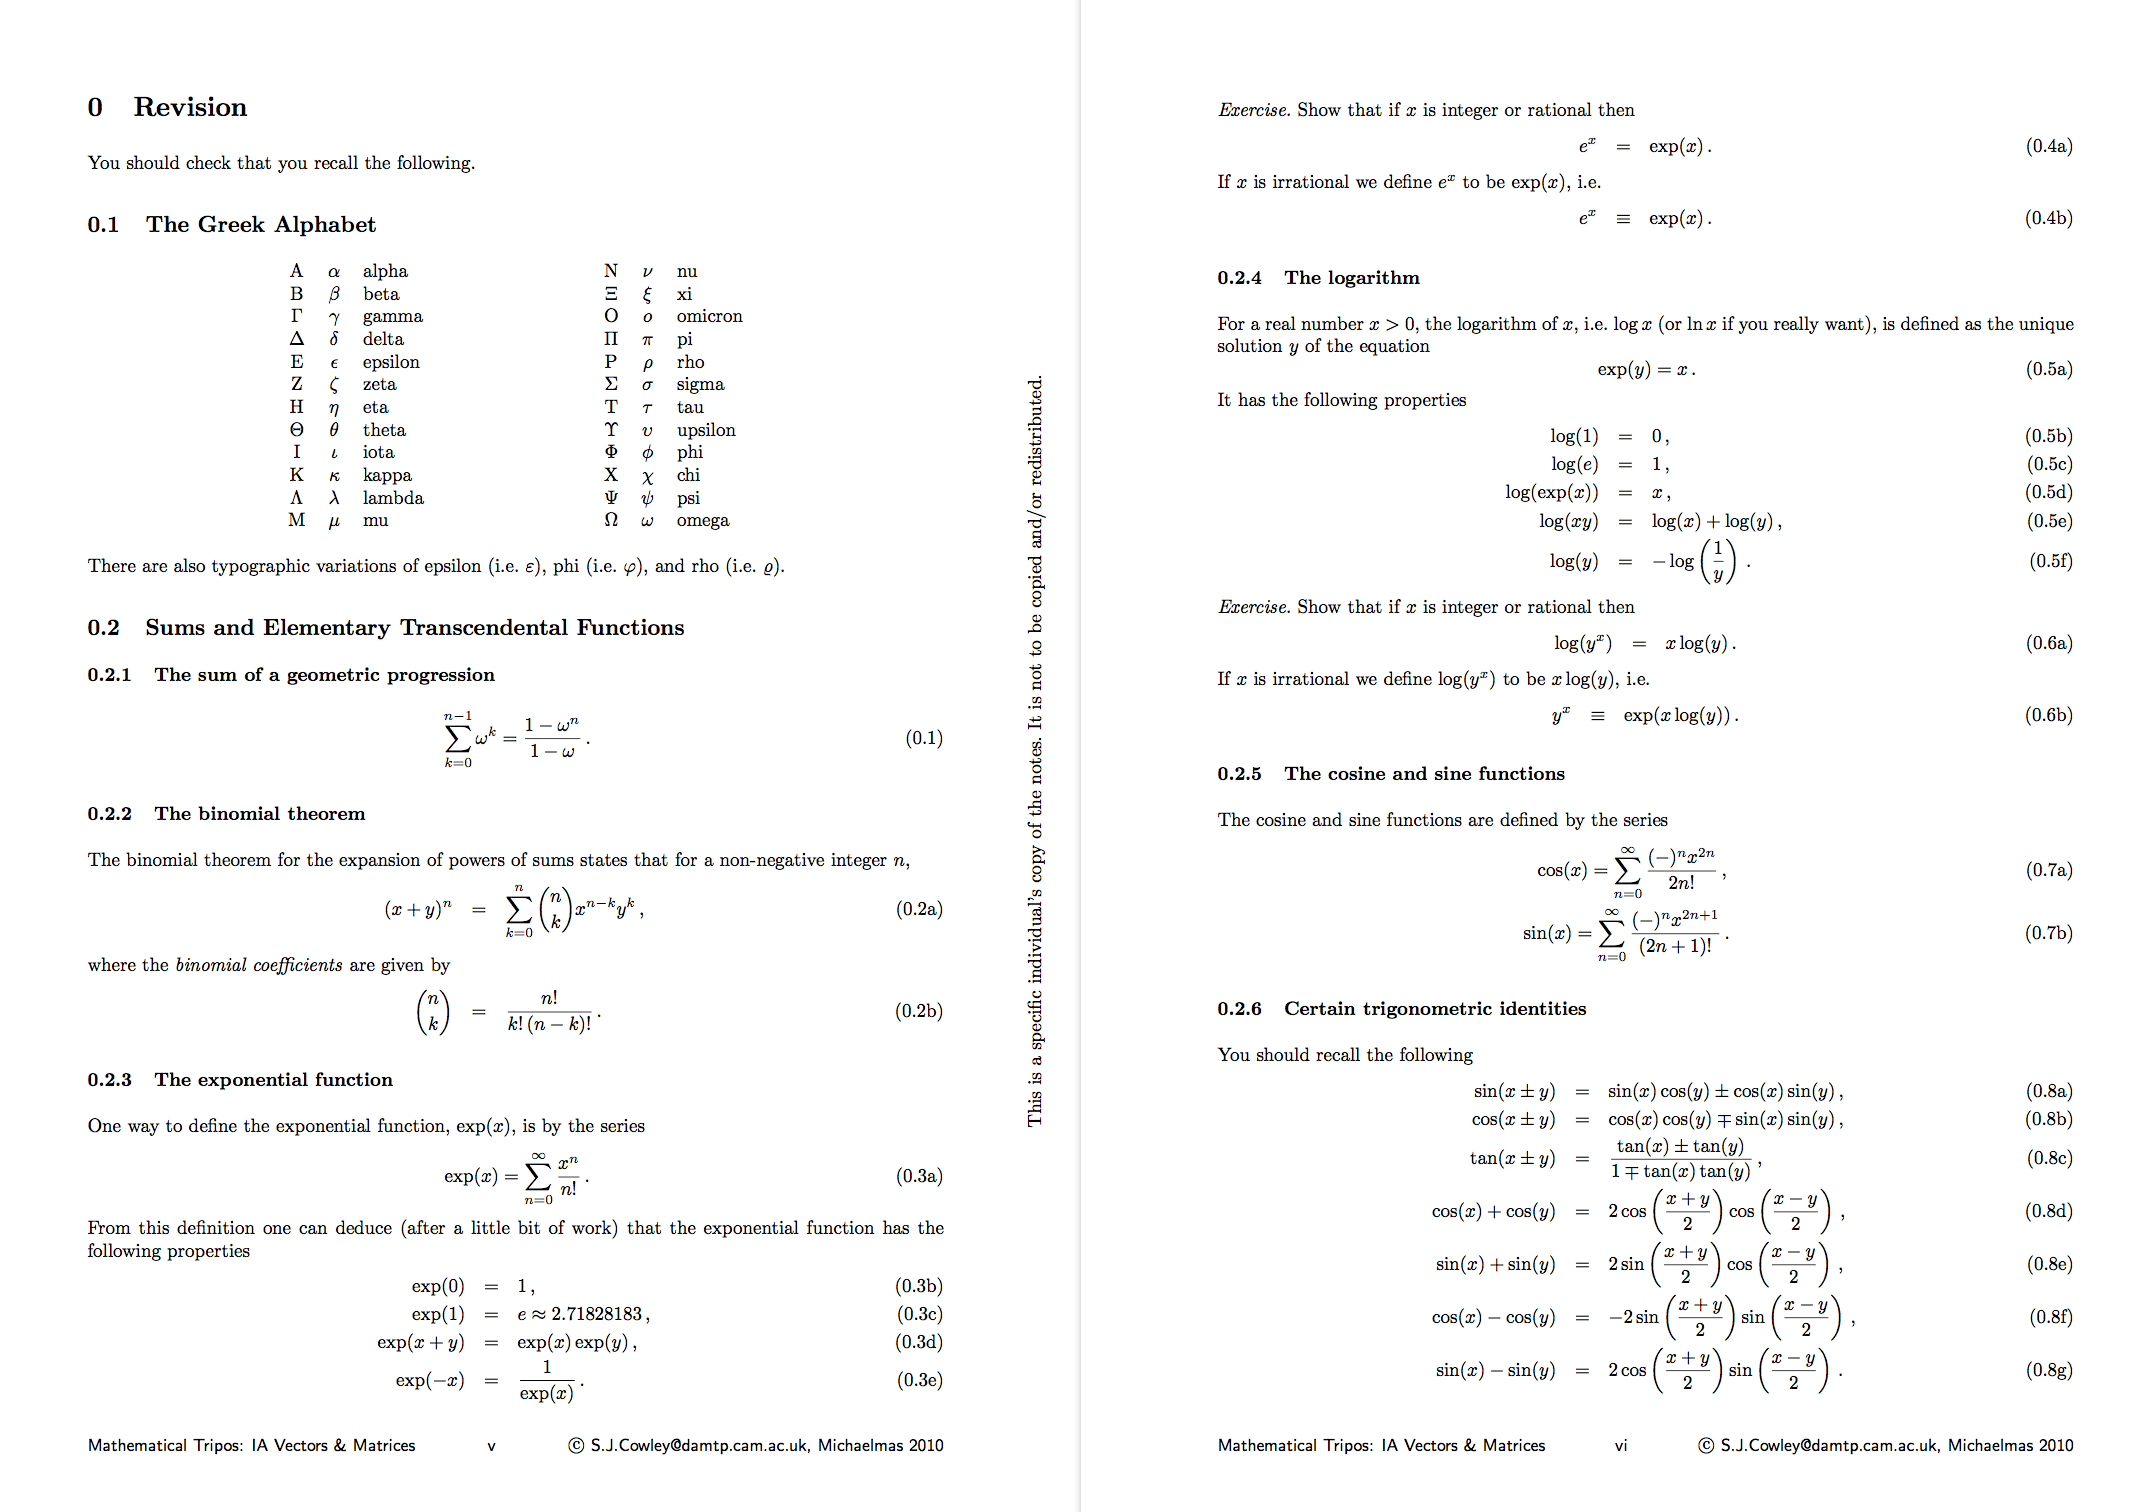
\includegraphics[width=400pt]{img/misc--cambridge-1a-vectors-and-matrices-revision-1.png}
\end{mdframed}
\begin{mdframed}
  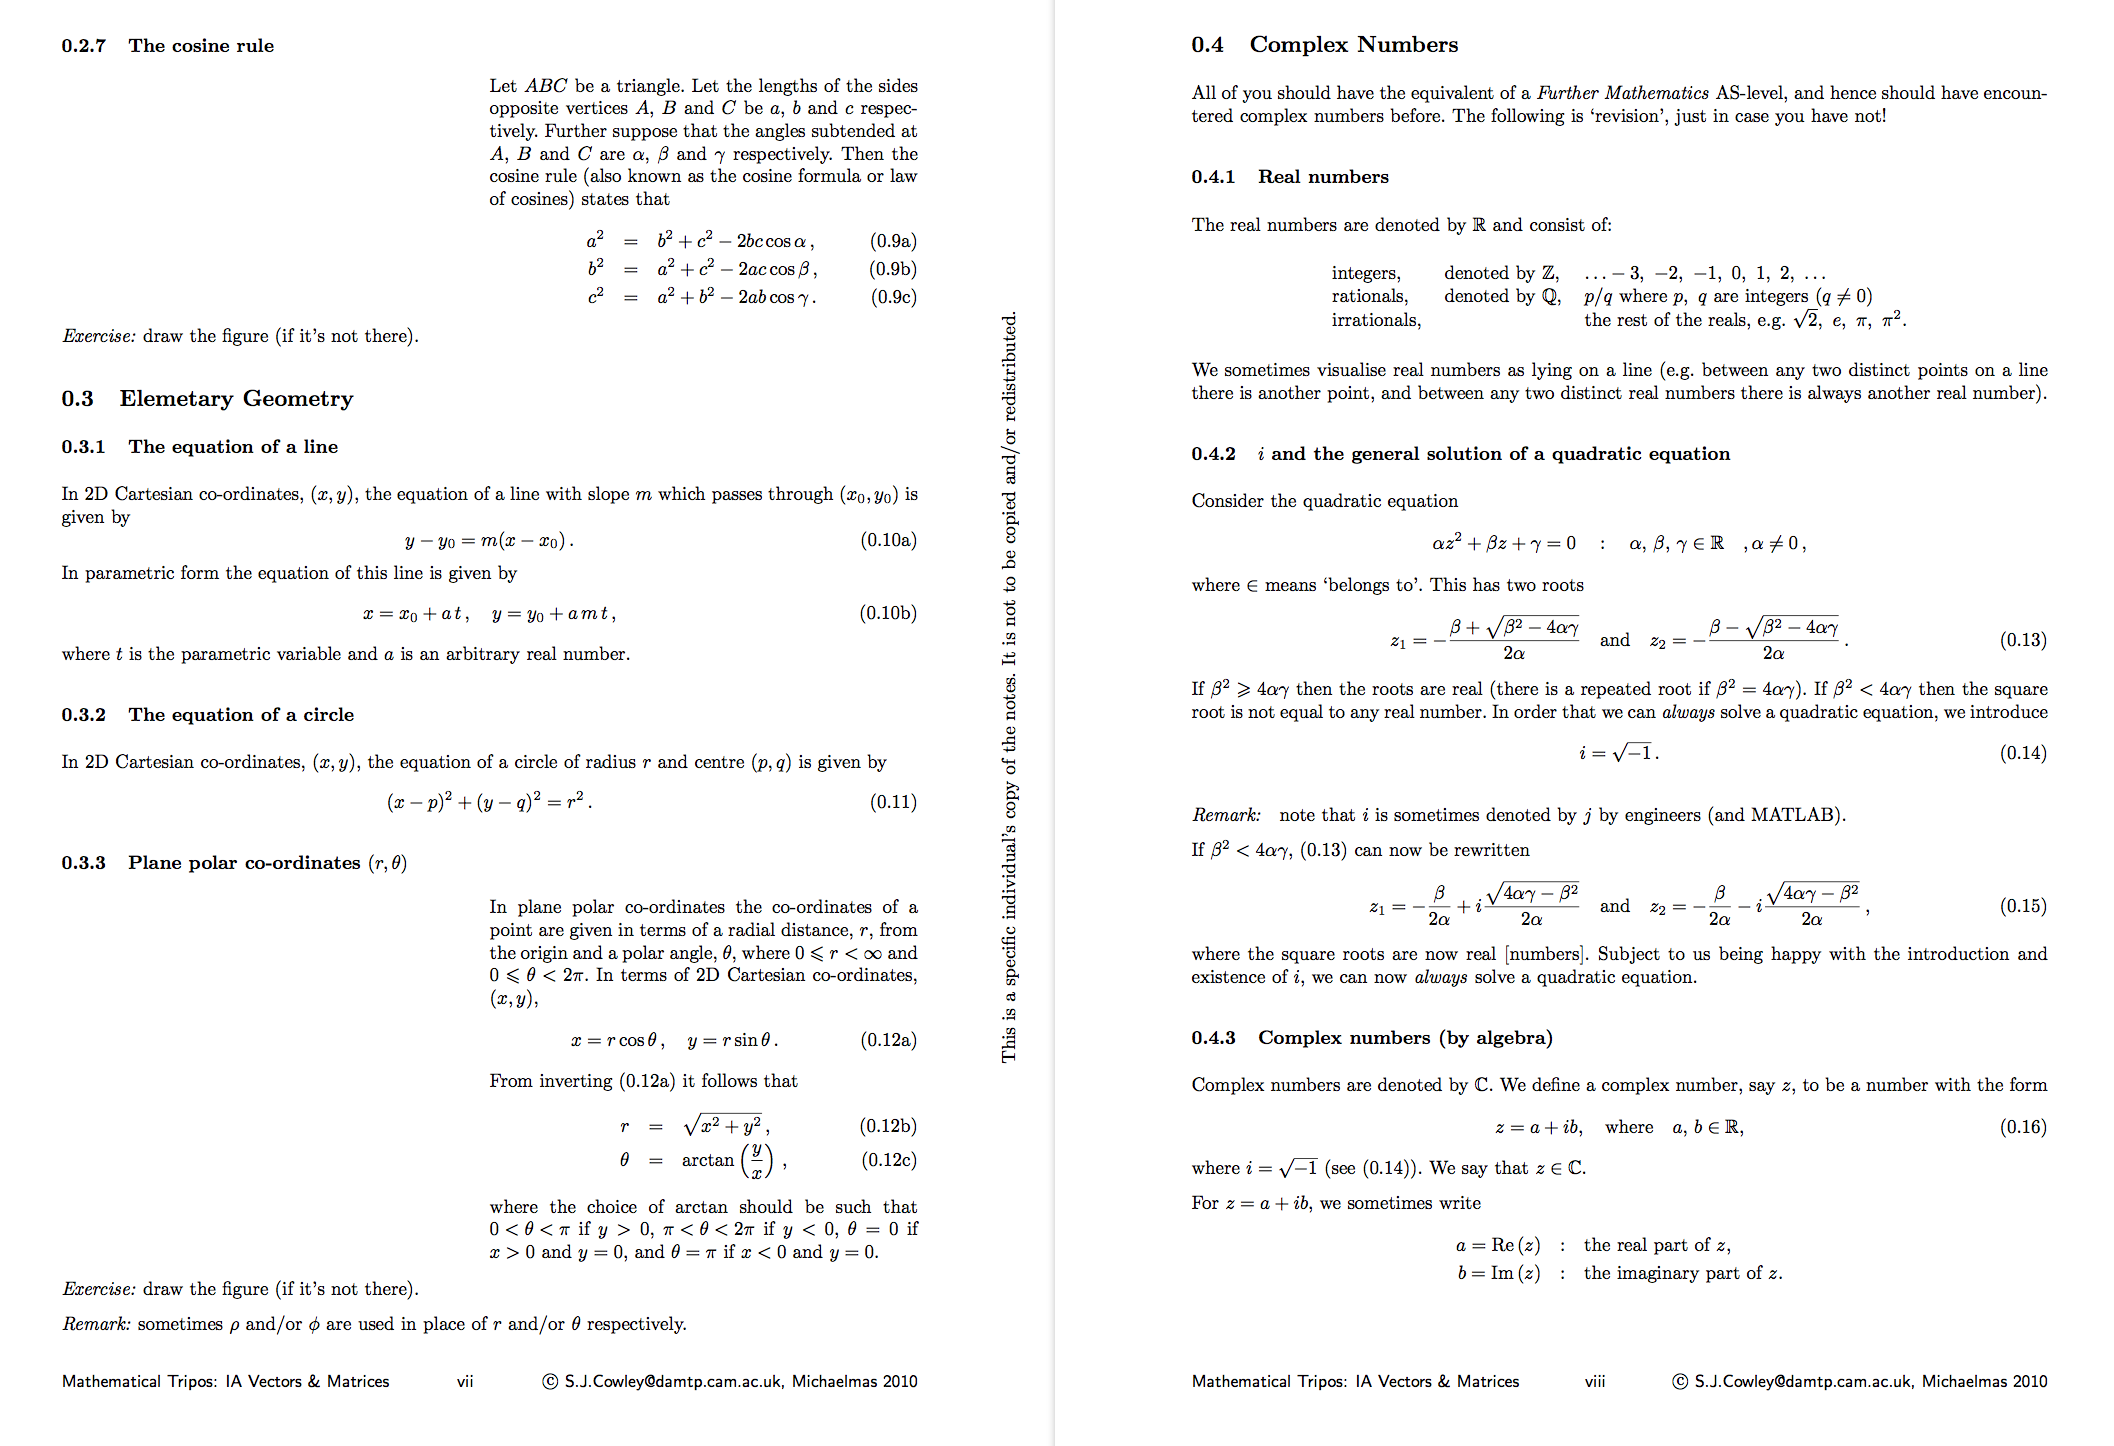
\includegraphics[width=400pt]{img/misc--cambridge-1a-vectors-and-matrices-revision-2.png}
\end{mdframed}
\begin{mdframed}
  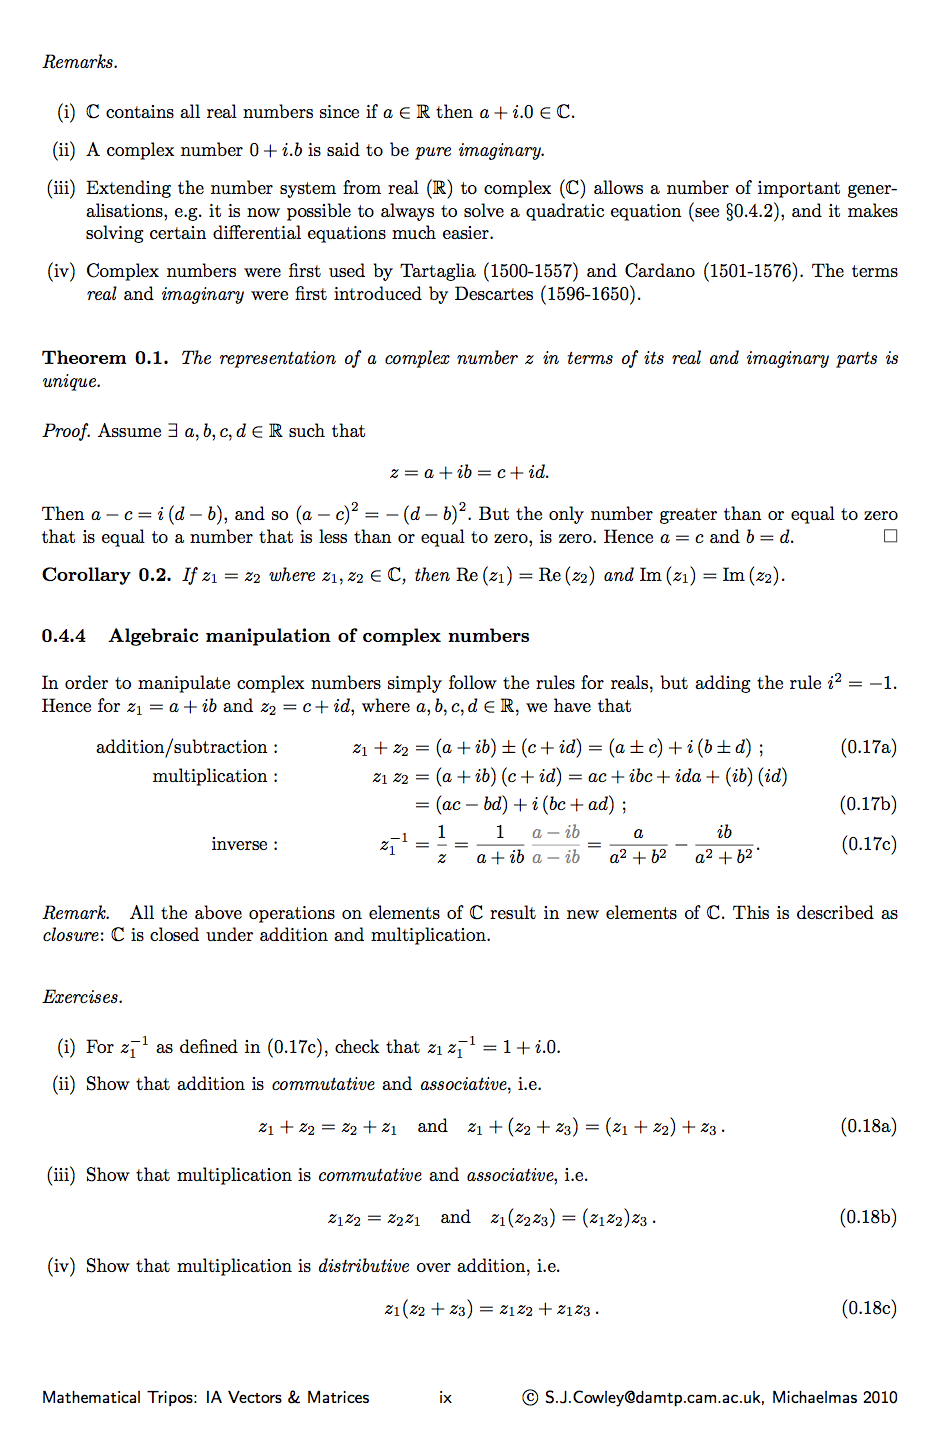
\includegraphics[width=400pt]{img/misc--cambridge-1a-vectors-and-matrices-revision-3.png}
\end{mdframed}